\documentclass[11pt, oneside]{article}   	% use "amsart" instead of "article" for AMSLaTeX format
\usepackage{geometry}                		% See geometry.pdf to learn the layout options. There are lots.
\geometry{letterpaper}                   		% ... or a4paper or a5paper or ... 
%\geometry{landscape}                		% Activate for rotated page geometry
\usepackage[parfill]{parskip}    		% Activate to begin paragraphs with an empty line rather than an indent
\usepackage{graphicx}				% Use pdf, png, jpg, or eps§ with pdflatex; use eps in DVI mode
								% TeX will automatically convert eps --> pdf in pdflatex		
\usepackage{caption}
\usepackage{subcaption}
\usepackage{float}
\usepackage{amssymb}
\usepackage{amsmath}
\usepackage{bm}
\usepackage{bbm}
\usepackage{mleftright}
\usepackage{todonotes}

\graphicspath{ {images/} }

\newcommand{\sotodo}{\todo[color=green]}
\newcommand{\sotodoinline}{\todo[color=green,inline=true]}
\newcommand{\bstodo}{\todo[color=pink]}
\newcommand{\bstodoinline}{\todo[color=pink,inline=true]}


%SetFonts

%SetFonts

\usepackage{natbib}
\usepackage{url}
%\bibliographystyle{elsarticle-harv}
\bibliographystyle{plain}

\newcommand{\half}{\frac{1}{2}}
\newcommand{\R}{\mathbb{R}}
\newcommand{\C}{\mathbb{C}}
\newcommand{\Z}{\mathbb{Z}}
\newcommand{\N}{\mathbb{N}}
\newcommand{\No}{\mathbb{N}_0}
\newcommand{\Ylm}{Y^m_l}
\newcommand{\Ylmfull}{Y^m_l(\theta,\varphi)}
\newcommand{\Plm}{P^m_l}
\newcommand{\costheta}{\cos\theta}
\newcommand{\sintheta}{\sin\theta}
\newcommand{\cosphi}{\cos\varphi}
\newcommand{\sinphi}{\sin\varphi}
\newcommand{\eimphi}{e^{im\varphi}}
\newcommand{\alphalm}{\alpha^m_l}
\newcommand{\clm}{c^m_l}
\newcommand{\ctilde}{\tilde{c}^m_l}
\newcommand{\ctildemod}{\tilde{c}^{|m|}_l}
\newcommand{\chat}{\hat{c}^m_l}
\newcommand{\chatmod}{\hat{c}^{|m|}_l}
\newcommand{\ddx}{\frac{\mathrm{d}}{\mathrm{d}x}}
\newcommand{\dmdxm}{\frac{\mathrm{d}^m}{\mathrm{d}x^m}}

\newcommand{\Atilde}{\tilde{A}_{l,m}}
\newcommand{\Btilde}{\tilde{B}_{l,m}}
\newcommand{\Dtilde}{\tilde{D}_{l,m}}
\newcommand{\Etilde}{\tilde{E}_{l,m}}
\newcommand{\Ftilde}{\tilde{F}_{l,m}}
\newcommand{\Gtilde}{\tilde{G}_{l,m}}
\newcommand{\Alm}{A_{l,m}}
\newcommand{\Blm}{B_{l,m}}
\newcommand{\Dlm}{D_{l,m}}
\newcommand{\Elm}{E_{l,m}}
\newcommand{\Flm}{F_{l,m}}
\newcommand{\Glm}{G_{l,m}}

\newcommand{\xione}{\xi^{(1)}_{n, \lambda}}
\newcommand{\xitwo}{\xi^{(2)}_{n, \lambda}}
\newcommand{\xithree}{\xi^{(3)}_{n, \lambda}}
\newcommand{\xifour}{\xi^{(4)}_{n, \lambda}}

\newcommand{\bigP}{\mathbb{P}}
\newcommand{\Pl}{\mathbb{P}_l}
\newcommand{\gradP}{T\mathbb{P}}
\newcommand{\gradPl}{T\mathbb{P}_l}
\newcommand{\gradY}{\nabla Y}
\newcommand{\gradYlm}{\nabla Y^m_l}
\newcommand{\gradpY}{\nabla^\perp Y}
\newcommand{\gradpYlm}{\nabla^\perp Y^m_l}

\newcommand{\Dlt}{D^T_l}

\newcommand{\curlyy}{\bm{\mathcal{Y}}}
\newcommand{\blone}{\beta_{l, 1}}
\newcommand{\blzero}{\beta_{l, 0}}
\newcommand{\blmone}{\beta_{l, -1}}
\newcommand{\chivec}{\bm{\chi}_{1,m_s}}
\newcommand{\cgcoeff}{\mathcal{C}}

\newcommand{\alm}{a_{l,m}}
\newcommand{\blm}{b_{l,m}}
\newcommand{\dlm}{d_{l,m}}
\newcommand{\elm}{e_{l,m}}
\newcommand{\flm}{f_{l,m}}
\newcommand{\glm}{g_{l,m}}
\newcommand{\hlm}{h_{l,m}}
\newcommand{\jlm}{j_{l,m}}
\newcommand{\klm}{k_{l,m}}
\newcommand{\almperp}{a_{l,m}^\perp}
\newcommand{\blmperp}{b_{l,m}^\perp}
\newcommand{\dlmperp}{d_{l,m}^\perp}
\newcommand{\elmperp}{e_{l,m}^\perp}
\newcommand{\flmperp}{f_{l,m}^\perp}
\newcommand{\glmperp}{g_{l,m}^\perp}
\newcommand{\hlmperp}{h_{l,m}^\perp}
\newcommand{\jlmperp}{j_{l,m}^\perp}
\newcommand{\klmperp}{k_{l,m}^\perp}

\newcommand{\unitvec}{\hat{\bm{k}}}

\newcommand{\Pnk}{P_{n,k}}
\newcommand{\Pab}{P^{(a,b)}}
\newcommand{\Pnkab}{P_{n,k}^{(a,b)}}
\newcommand{\Wab}{{W^{(a,b)}}}
\newcommand{\Pmjab}{P_{m,j}^{(a,b)}}
\newcommand{\alphaab}{\alpha^{(a,b)}}
\newcommand{\betaab}{\beta^{(a,b)}}
\newcommand{\bigPab}{\bigP^{(a,b)}}
\newcommand{\Dnt}{D^T_n}
\newcommand{\Wii}{W^{(1,1)}}
\newcommand{\Pii}{P^{(1,1)}}
\newcommand{\bigPii}{{\mathbb{P}^{(1,1)}}}
\newcommand{\Poo}{P^{(0,0)}}
\newcommand{\bigPoo}{{\mathbb{P}^{(0,0)}}}
\newcommand{\Poi}{P^{(0,1)}}
\newcommand{\Pio}{P^{(1,0)}}
\newcommand{\dx}{\frac{\partial}{\partial x}}
\newcommand{\dy}{\frac{\partial}{\partial y}}
\newcommand{\element}{\tau}
\newcommand{\refelement}{\hat{\tau}}
\newcommand{\FEset}{\mathcal{T}}
\newcommand{\bigW}{\mathbb{W}}
\newcommand{\bigWab}{\mathbb{W}^{(a,b)}}
\newcommand{\bigWii}{{\mathbb{W}^{(1,1)}}}
\newcommand{\bigQ}{\mathbb{Q}}
\newcommand{\bigQab}{\bigQ^{(a,b)}}

\usepackage{amsthm}

\newtheorem{proposition}{Proposition}
\newtheorem{lemma}{Lemma} 
\newtheorem{theorem}{Theorem} 
\newtheorem{definition}{Definition}


\def\addtab#1={#1\;&=}

\def\meeq#1{\def\ccr{\\\addtab}
%\tabskip=\@centering
 \begin{align*}
 \addtab#1
 \end{align*}
  }  
  
  \def\leqaddtab#1\leq{#1\;&\leq}
  \def\mleeq#1{\def\ccr{\\\addtab}
%\tabskip=\@centering
 \begin{align*}
 \leqaddtab#1
 \end{align*}
  }  


\def\vc#1{\mbox{\boldmath$#1$\unboldmath}}

\def\vcsmall#1{\mbox{\boldmath$\scriptstyle #1$\unboldmath}}

\def\vczero{{\mathbf 0}}


%\def\beginlist{\begin{itemize}}
%
%\def\endlist{\end{itemize}}


\def\pr(#1){\left({#1}\right)}
\def\br[#1]{\left[{#1}\right]}
\def\fbr[#1]{\!\left[{#1}\right]}
\def\set#1{\left\{{#1}\right\}}
\def\ip<#1>{\left\langle{#1}\right\rangle}
\def\iip<#1>{\left\langle\!\langle{#1}\right\rangle\!\rangle}

\def\norm#1{\left\| #1 \right\|}

\def\abs#1{\left|{#1}\right|}
\def\fpr(#1){\!\pr({#1})}

\def\Re{{\rm Re}\,}
\def\Im{{\rm Im}\,}

\def\floor#1{\left\lfloor#1\right\rfloor}
\def\ceil#1{\left\lceil#1\right\rceil}


\def\mapengine#1,#2.{\mapfunction{#1}\ifx\void#2\else\mapengine #2.\fi }

\def\map[#1]{\mapengine #1,\void.}

\def\mapenginesep_#1#2,#3.{\mapfunction{#2}\ifx\void#3\else#1\mapengine #3.\fi }

\def\mapsep_#1[#2]{\mapenginesep_{#1}#2,\void.}


\def\vcbr[#1]{\pr(#1)}


\def\bvect[#1,#2]{
{
\def\dots{\cdots}
\def\mapfunction##1{\ | \  ##1}
	\sopmatrix{
		 \,#1\map[#2]\,
	}
}
}

\def\vect[#1]{
{\def\dots{\ldots}
	\vcbr[{#1}]
}}

\def\vectt[#1]{
{\def\dots{\ldots}
	\vect[{#1}]^{\top}
}}

\def\Vectt[#1]{
{
\def\mapfunction##1{##1 \cr} 
\def\dots{\vdots}
	\begin{pmatrix}
		\map[#1]
	\end{pmatrix}
}}



\def\thetaB{\mbox{\boldmath$\theta$}}
\def\zetaB{\mbox{\boldmath$\zeta$}}


\def\newterm#1{{\it #1}\index{#1}}


\def\TT{{\mathbb T}}
\def\C{{\mathbb C}}
\def\R{{\mathbb R}}
\def\II{{\mathbb I}}
\def\F{{\mathcal F}}
\def\E{{\rm e}}
\def\I{{\rm i}}
\def\D{{\rm d}}
\def\dx{\D x}
\def\dy{\D y}
\def\CC{{\cal C}}
\def\DD{{\cal D}}
\def\U{{\mathbb U}}
\def\A{{\cal A}}
\def\K{{\cal K}}
\def\DTU{{\cal D}_{{\rm T} \rightarrow {\rm U}}}
\def\LL{{\cal L}}
\def\B{{\cal B}}
\def\T{{\cal T}}
\def\W{{\cal W}}


\def\tF_#1{{\tt F}_{#1}}
\def\Fm{\tF_m}
\def\Fab{\tF_{\alpha,\beta}}
\def\FC{\T}
\def\FCpmz{\FC^{\pm {\rm z}}}
\def\FCz{\FC^{\rm z}}

\def\tFC_#1{{\tt T}_{#1}}
\def\FCn{\tFC_n}

\def\rmz{{\rm z}}

\def\chapref#1{Chapter~\ref{Chapter:#1}}
\def\secref#1{Section~\ref{Section:#1}}
\def\exref#1{Exercise~\ref{Exercise:#1}}
\def\lmref#1{Lemma~\ref{Lemma:#1}}
\def\propref#1{Proposition~\ref{Proposition:#1}}
\def\warnref#1{Warning~\ref{Warning:#1}}
\def\thref#1{Theorem~\ref{Theorem:#1}}
\def\defref#1{Definition~\ref{Definition:#1}}
\def\probref#1{Problem~\ref{Problem:#1}}
\def\corref#1{Corollary~\ref{Corollary:#1}}
\def\appref#1{Appendix~\ref{Appendix:#1}}

\def\sgn{{\rm sgn}\,}
\def\Ai{{\rm Ai}\,}
\def\Bi{{\rm Bi}\,}
\def\wind{{\rm wind}\,}
\def\erf{{\rm erf}\,}
\def\erfc{{\rm erfc}\,}
\def\qqquad{\qquad\quad}
\def\qqqquad{\qquad\qquad}


\def\spand{\hbox{ and }}
\def\spodd{\hbox{ odd}}
\def\speven{\hbox{ even}}
\def\qand{\quad\hbox{and}\quad}
\def\qqand{\qquad\hbox{and}\qquad}
\def\qfor{\quad\hbox{for}\quad}
\def\qqfor{\qquad\hbox{for}\qquad}
\def\qas{\quad\hbox{as}\quad}
\def\qqas{\qquad\hbox{as}\qquad}
\def\qor{\quad\hbox{or}\quad}
\def\qqor{\qquad\hbox{or}\qquad}
\def\qqwhere{\qquad\hbox{where}\qquad}



%%% Words

\def\naive{na\"\i ve\xspace}
\def\Jmap{Joukowsky map\xspace}
\def\Mobius{M\"obius\xspace}
\def\Holder{H\"older\xspace}
\def\Mathematica{{\sc Mathematica}\xspace}
\def\apriori{apriori\xspace}
\def\WHf{Weiner--Hopf factorization\xspace}
\def\WHfs{Weiner--Hopf factorizations\xspace}

\def\Jup{J_\uparrow^{-1}}
\def\Jdown{J_\downarrow^{-1}}
\def\Jin{J_+^{-1}}
\def\Jout{J_-^{-1}}



\def\bD{\D\!\!\!^-}




\def\questionequals{= \!\!\!\!\!\!{\scriptstyle ? \atop }\,\,\,}

\def\elll#1{\ell^{\lambda,#1}}
\def\elllp{\ell^{\lambda,p}}
\def\elllRp{\ell^{(\lambda,R),p}}


\def\elllRpz_#1{\ell_{#1{\rm z}}^{(\lambda,R),p}}


\def\sopmatrix#1{\begin{pmatrix}#1\end{pmatrix}}

\def\socases#1{\begin{cases} #1 \end{cases}}


\def\Problem#1#2\par{\begin{problem}\label{pb:#1} #2\end{problem}}
\def\Theorem#1#2\par{\begin{theorem}\label{th:#1} #2\end{theorem}}
\def\Conjecture#1#2\par{\begin{conjecture}\label{conj:#1} #2\end{conjecture}}
\def\Proposition#1#2\par{\begin{proposition}\label{prop:#1} #2\end{proposition}}
\def\Definition#1#2\par{\begin{definition}\label{def:#1} #2\end{definition}}
\def\Corollary#1#2\par{\begin{corollary}\label{cr:#1} #2\end{corollary}}
\def\Lemma#1#2\par{\begin{lemma}\label{lm:#1} #2\end{lemma}}
\def\Example#1#2\par{\begin{example}\label{ex:#1} #2\end{example}}
\def\Remark #1\par{\begin{remark*}#1\end{remark*}}


\def\Proof{\begin{proof}}
\def\mqed{\end{proof}}


\def\Figuretwow[#1,#2]#3#4\par{
\begin{figure}[tb]
\begin{center}{
\includegraphics[width=#3]{Figures/#1}\includegraphics[width=#3]{Figures/#2}}
\end{center}
\caption{#4}\label{fig:#1} 
\end{figure}
}

%\usepackage{media9}
%\graphicspath{ {../sphere/plots} }



\title{Sparse spectral and $p$-finite element methods on disk-slices and rhombi I: zero boundary conditions}
\author{Sheehan Olver, Ben Snowball}
%\date{}							% Activate to display a given date or no date


\begin{document}

\maketitle

\begin{abstract}
In recent years, sparse spectral methods have been derived using hierarchies of classical orthogonal polynomials on intervals, disks, and triangles. In this work we extend this methodology to a hierarchy of non-classical orthogonal polynomials on disk slices (e.g. a half disk) and rhombi. This builds on the observation that sparsity is guaranteed due to the boundary being defined by an algebraic curve, and that the entries of partial differential operators can be determined using formulae in terms of (non-classical) univariate orthogonal polynomials. 
\end{abstract}


%
\section{Introduction}

This paper develops sparse spectral methods for solving linear partial differential equations on a special class of geometries that includes disk slices and rhombi.  
More precisely, let  \(\rho \: : \: (\alpha,\beta) \: \to (0,\infty)\) be such that either:

\begin{enumerate}
\item  \(\rho\) is a degree 1 polynomial, or 
\item \(\rho\) is the square root of a non-negative degree \(\le\) 2 polynomial, \(-\gamma = \delta > 0\), and \(w_2\) is an even function.
\end{enumerate}

We consider the solution of partial differential equations on the domain
\begin{align}
\Omega := \{(x,y) \in \R^2 \quad | \quad \alpha < x < \beta, \: \gamma \rho(x) < y < \delta \rho(x)\}
\end{align}
For simplicity of discussion we focus on the half-disk, where $\rho(x) = \sqrt{1-x^2}$,  $(\alpha,\beta) = (0, 1)$, and  $(\gamma, \delta)  = (-1,1)$, with discussion of extension to other geometries in the appendix. 


We show that partial differential equations become sparse linear systems when viewed as acting on expansions involving a family of orthogonal polynomials that  generalise Jacobi polynomials, mirroring the ultraspherical spectral method for ordinary differential equations \cite{SOATUltraspherical} and its analogue on the triangle \cite{SOATGVTriangle}.  On the half-disk the family of weights we consider are of the form
$$
W^{(a,b)}(x,y) = x^a (1-x-y)^b
$$
with corresponding OPs denoted $P_{n,k}^{(a,b)}(x,y)$. Sparsity comes from expanding the domain and range of an operator  using different polynomials. Where the sparsity pattern and entries derived in \cite{SOATGVTriangleRecurrence,SOATGVTriangle}  results from manipulations of Jacobi polynomials, in the present work we use a more general integration-by-parts argument to deduce the sparsity structure, alongside quadrature rules to determine the entries.  Furthermore, we use this framework to derive sparse $p$-finite element methods that are analogous to those of Beuchler and Sch\"oberl on tetrahedra \cite{TriangleFEM}. 

The motivation for this work is solving partial differential equations on sub-domains of the sphere. In particular, OPs on a half-sphere can be represented using two families of OPs on the half-disk. Constructing sparse spectral methods for surface PDEs on half-spheres, spherical caps, and spherical triangles is future work, and has applications in weather prediction. Other extensions include a full $hp$-finite element method on sections of a disk, which has applications in fluids. 

  

 We present our procedure  to gain a (two-parameter) family of 2D orthogonal polynomials (OPs) on the half disk domain, by combining 1D OPs to the interval, to form 2D OPs on the disk. We will derive a quadrature rule on the half disk that can be used to expand a function in the OP basis up to a given order. We will demonstrate that these families will have sparse operators (including Jacobi operators representing multiplication by $x$ and $y$, and partial differential operators), and how we can implement function evaluation using the coefficients of the expansion of a given function using the Clenshaw algorithm. We can extend this work directly by projecting up to 3D OPs on the hemisphere, where sparse operators, function evaluation and expansion etc. can be found similarly. 

\section{Orthogonal polynomials on the half disk}

In this section we outline some basic properties of $P_{n,k}^{(a,b)}(x,y)$. The symmetry in the weight allows us to express the polynomials in terms of 1D OPs, and deduce certain properties such as recurrence relationships. 

\subsection{Explicit construction}


By using a similar process to \cite[p55--56]{dunkl2014orthogonal} we can construct 2D orthogonal polynomials on $\Omega$ from 1D orthogonal polynomials on the intervals \([0,1]\) and \([-1,1]\).

\begin{proposition}
Let \(w_1 : (\alpha,\beta) \: \to \R\), \(w_2 : (\gamma,\delta) \: \to \R\) be weight functions with \(\alpha,\beta,\gamma,\delta \in \R\),
Then, \(\forall n,k = 0,1,2,\dots\) let \(\{p_{n,k}\}\) be polynomials orthogonal with respect to the weight \(\rho(x)^{2k+1} w_1(x)\), and \(\{q_{n}\}\) be polynomials orthogonal with respect to the weight \(w_2(x)\). Then
$$
\Pnk(x,y) := p_{n-k,k}(x) \: \rho(x)^k \: q_k(\frac{y}{\rho(x)}) \qquad\hbox{for} \qquad 0 \le k \le n, \: n = 0,1,2,\dots
$$
are orthogonal polynomials with respect to the weight \(W(x,y) := w_1(x) \: w_2(\frac{y}{\rho(x)}) \) on $\Omega$. 
\end{proposition}

For the half disk, the weight $W^{(a,b)}(x,y) = x^a \: (1-x^2-y^2)^b$ results from setting:

\begin{align}
\begin{cases}
(\alpha,\beta) &:= (0.1) \\
(\gamma,\delta) &:= (-1,1) \\
\rho(x) &:= (1-x^2)^{\half} \\
w_1(x) &:= x^a \: (1-x^2)^b \\
w_2(x) &:= (1-x^2)^b = (1-x)^b \: (1+x)^b,
\end{cases}
\end{align}

The weight $w_2(x)$ is an ultraspherical weight, and the corresponding OPs are   the Jacobi polynomials  \(\{P_n^{(b, b)}\}\). The weight $w_1(x)$ is non-classical and we introduce the notation \(\{H_n^{(a, b)}\}\) for the orthonormal polynomials. Thus we arrive at  a two parameter family of  2D orthogonal polynomials \(\{\Pnk\}\) given by, for \(0 \le k \le n, \: n = 0,1,2,\dots,\)
\begin{align}
 \Pnk^{(a,b)}(x,y) := H_{n-k}^{(a, b+k+\half)}(x) \: \rho(x)^k \: P_k^{(b,b)}(\frac{y}{\rho(x)}), \quad (x,y) \in \Omega, 
\end{align}
orthogonal on \(\Omega\) with respect to the weight $W^{(a,b)}(x,y)$.


\subsection{Jacobi matrices}

Express the three-term recurrences associated to $H_n^{(a,b)}$ and $P_n^{(b,b)}$ as
\begin{align}
x H_n^{(a,b)}(x) &= \beta_n^{(a,b)} H_{n+1}^{(a,b)}(x) + \alpha_n^{(a,b)} H_n^{(a,b)}(x) + \beta_{n-1}^{(a,b)} H_{n-1}^{(a,b)}(x) \\
y P_n^{(b,b)}(y) &= \delta_n^{(b)} P_{n+1}^{(b,b)}(y) + \gamma_n^{(b)} P_n^{(b,b)}(y) + \delta_{n-1}^{(b)} P_{n-1}^{(b,b)}(y),
\end{align}
where we note that \(\gamma_n^{(b)} = 0\) \(\forall n = 0,1,2,\dots\). We can use these to determine the 2D recurences for $P_{n,k}^{(a,b)}(x,y)$:

\begin{lemma}
$\Pnk^{(a,b)}(x,y)$ satisfy the following 3-term recurrences:
\begin{align}
x \Pnk^{(a,b)}(x,y) &= \alphaab_{n,k,1} \: P_{n-1, k}^{(a,b)}(x, y) + \alphaab_{n,k,2} \: P_{n, k}^{(a,b)}(x, y) + \alphaab_{n+1,k,1} \: P_{n+1, k}^{(a,b)}(x, y), \\
y \Pnk^{(a,b)}(x,y) &= \betaab_{n,k,1} \: P_{n-1, k-1}^{(a,b)}(x, y) + \betaab_{n,k,2} \: P_{n-1, k+1}^{(a,b)}(x, y) \nonumber \\
		& \quad \quad + \betaab_{n,k,3} \: P_{n, k-1}^{(a,b)}(x, y) + \betaab_{n,k,4} \: P_{n, k+1}^{(a,b)}(x, y) \nonumber \\
		& \quad \quad + \betaab_{n,k,5} \: P_{n+1, k-1}^{(a,b)}(x, y) + \betaab_{n,k,6} \: P_{n+1, k+1}^{(a,b)}(x, y),
\end{align}
for \((x,y) \in \Omega\), where
\begin{align}
\alphaab_{n,k,1} &:= \beta_{n-k-1}^{(a, b+k+\half)} \\
\alphaab_{n,k,2} &:= \alpha_{n-k}^{(a, b+k+\half)} \\
\betaab_{n,k,1} &:= \frac{\delta_{k-1}^{(b)}}{|| P_{n-1,k-1}^{(a,b)} ||_{W^{(a,b)}}^2} \: \ip<H_{n-k}^{(a, b+k+\half)}, H_{n-k}^{(a, b+k-\half)}>_{H^{(a, b+k+\half)}} \\
\betaab_{n,k,2} &:= \frac{\delta_{k}^{(b)}}{|| P_{n-1,k+1}^{(a,b)} ||_{W^{(a,b)}}^2} \: \ip<H_{n-k}^{(a, b+k+\half)}, H_{n-k-2}^{(a, b+k+\frac{3}{2})}>_{H^{(a, b+k+\frac{3}{2})}} \\
\betaab_{n,k,3} &:= \frac{\delta_{k-1}^{(b)}}{|| P_{n,k-1}^{(a,b)} ||_{W^{(a,b)}}^2} \: \ip<H_{n-k}^{(a, b+k+\half)}, H_{n-k+1}^{(a, b+k-\half)}>_{H^{(a, b+k+\half)}} \\
\betaab_{n,k,4} &:= \frac{\delta_{k}^{(b)}}{|| P_{n,k+1}^{(a,b)} ||_{W^{(a,b)}}^2} \: \ip<H_{n-k}^{(a, b+k+\half)}, H_{n-k-1}^{(a, b+k+\frac{3}{2})}>_{H^{(a, b+k+\frac{3}{2})}} \\
\betaab_{n,k,5} &:= \frac{\delta_{k-1}^{(b)}}{|| P_{n+1,k-1}^{(a,b)} ||_{W^{(a,b)}}^2} \: \ip<H_{n-k}^{(a, b+k+\half)}, H_{n-k+2}^{(a, b+k-\half)}>_{H^{(a, b+k+\half)}} \\
\betaab_{n,k,6} &:= \frac{\delta_{k}^{(b)}}{|| P_{n+1,k+1}^{(a,b)} ||_{W^{(a,b)}}^2} \: \ip<H_{n-k}^{(a, b+k+\half)}, H_{n-k}^{(a, b+k+\frac{3}{2})}>_{H^{(a, b+k+\frac{3}{2})}}. 
\end{align}
where $|| p(x,y) ||_{W^{(a,b)}}^2 := \int_\Omega p(x,y)^2 \: \Wab(x,y) \: d\mathbf{x}$ and $\ip<p(x), q(x)>_{H^{(a, b)}} := \int_\alpha^\beta p(x) \: q(x) \: x^a \: (1-x^2)^b \: dx$, i.e the 1D inner product using the $\{H^{(a,b)}_n\}$ family weight.

\end{lemma}

\begin{proof}
Note that \(\ip<y \Pnkab, P_{m,j}^{(a,b)}>_\Wab = 0\) for \(m < n-1\) (and for \(m > n+2\)). Thus for \(m = n-1, n, n+1,\) \(j = 0,\dots,m:\)
\begin{align}
\ip<y \Pnkab, P_{m,j}^{(a,b)}>_\Wab &= \int \int_\Omega \Pnkab(x,y) \: \Pmjab(x,y) \: y \: \Wab(x,y) \: dy \: dx \\
&= \Big( \int^1_0 H_{n-k}^{(a, b+k+\half)}(s) \: H_{m-j}^{(a, b+j+\half)}(s) \: s^a \: \rho(s)^{2b+k+j+2} \: ds \Big) \nonumber \\
& \quad \quad \quad\cdot \: \Big( \int^1_{-1} P_k^{(b,b)}(t) \: P_j^{(b,b)}(t) \: t \: (1-t^2)^b \: dt \Big) \\
&= \begin{cases}
    	\delta_k^{(b)} \: \ip<H_{n-k}^{(a, b+k+\half)}, H_{m-k-1}^{(a, b+k+\frac{3}{2})}>_{H^{(a, b+k+\frac{3}{2})}} \quad& \text{if } j = k+1 \\
	\delta_{k-1}^{(b)} \: \ip<H_{n-k}^{(a, b+k+\half)}, H_{m-k+1}^{(a, b+k-\half)}>_{H^{(a, b+k+\half)}} \quad& \text{if } j = k-1 \\
	0 & \text{otherwise}
      \end{cases}.
\end{align}

\end{proof}


Three-term recurrences lead to Jacobi operators that correspond to multiplication by $x$ and $y$. Define, for some $N \in \No$:
\begin{align}
\bigPab_n := \begin{bmatrix}
		P^{(a,b)}_{n,-n}(x,y) \\
		\vdots \\
		P^{(a,b)}_{n,n}(x,y)
	\end{bmatrix} \in \R^{n+1}, 
\quad \quad 
\bigPab := \begin{bmatrix}
		\bigPab_0 \\
		\bigPab_1 \\
		\vdots \\
		\bigPab_N
	\end{bmatrix}
\end{align}
and set \(J_x^{(a,b)}, J_y^{(a,b)}\) as the \(\half (N+1)(N+2) \times \half (N+1)(N+2)\) Jacobi matrices corresponding to
\begin{align}
J_x^{(a,b)} \bigPab(x,y) = x \bigPab(x,y), \quad J_y^{(a,b)} \bigPab(x,y) = y \bigPab(x,y).
\end{align}
Then  \(J_x^{(a,b)}, J_y^{(a,b)}\) have the Banded-Block-Banded structures
\begin{align}
J_{x/y}^{(a,b)} &= \begin{bmatrix}
		B^{x/y}_0 & A^{x/y}_0 & & & & \\
		C^{x/y}_1 & B^{x/y}_1 & A^{x/y}_1 & & & \\
		& C^{x/y}_2 & B^{x/y}_2 & A^{x/y}_2  & & & \\
		& & C^{x/y}_3 & \ddots & \ddots & \\
		& & & \ddots & \ddots & \ddots \\
	\end{bmatrix}
\end{align}
where
\begin{align}
A^x_n &:= \begin{bmatrix}
		\alphaab_{n+1,0,1} & 0 & \hdots & 0 \\
		& \ddots & & \vdots & \\
		& & \alphaab_{n+1,n,1} & 0 \\
	    \end{bmatrix} \in \R^{(n+1)\times(n+2)}, \quad n = 0,1,2,\dots,N-1 \\
B^x_n &:= \begin{bmatrix}
		\alphaab_{n,0,2} & & \\
		& \ddots & \\
		& & \alphaab_{n,n,2} \\
	    \end{bmatrix} \in \R^{(n+1)\times(n+1)} \quad n = 0,1,2,\dots,N \\
C^x_n &:= \big( A^x_n \big)^T \in \R^{(n+1)\times n},  \quad n = 1,2,\dots,N, \\ 
\nonumber \\
A^y_n &:= \begin{bmatrix}
		0 & \betaab_{n,0,6} & & & \\
		\betaab_{n,1,5} & 0 & & & \\
		& \ddots & \ddots & \ddots & \\
		& & \betaab_{n,n,5}& 0 & \betaab_{n,n,6} \\
	    \end{bmatrix} \in \R^{(n+1)\times(n+2)}, \quad n = 0,1,2,\dots,N-1 \\
B^y_n &:= \begin{bmatrix}
		0 & \betaab_{n,0,4} & & \\
		\betaab_{n,1,3} & 0 & \ddots & \\
		& \ddots & \ddots & \betaab_{n,n-1,4} \\
		& & \betaab_{n,n,3} & 0
	    \end{bmatrix} \in \R^{(n+1)\times(n+1)}  \quad n = 0,1,2,\dots,N \\
C^y_n &:= \begin{bmatrix}
		0 & \betaab_{n,0,2} & & \\
		\betaab_{n,1,1} & 0 & \ddots & \\
		& \ddots & \ddots & \betaab_{n,n-2,2} \\
		& & \ddots & 0 \\
		& & & \betaab_{n,n,1} \\
	    \end{bmatrix} \in \R^{(n+1)\times n}, \quad n = 1,2,\dots,N.
\end{align}

Note that the sparsity of the Jacobi matrices (in particular the sparsity of the sub-blocks) comes from the natural sparsity of the three-term recurrences of the 1D OPs. In other words, sparsity is not dependent on the domain.




\subsection{Building the OPs} 

Combining each system in (71) we can write the block-tridiagonal system
\begin{align}
\renewcommand\arraystretch{1.3}
\mleft[
\begin{array}{cccc}
		1 & & & \\
		B_0-G_0(x,y) & A_0 & & \\
		C_1 & B_1-G_1(x,y) & \quad A_1 \quad & \\
		& C_2 & \ddots & \ddots \\
		& & \ddots &
\end{array}
\mright]
\bigPab(x,y)
=
\begin{bmatrix}
	P^{(a,b)}_{0,0} \\ 0 \\ 0 \\ \vdots \\ 0 \\
\end{bmatrix}.
\end{align}
where we note \(P^{(a,b)}_{0,0}(x,y) \equiv H_0^{(a,b)} \: P_0^{(b,b)}\), and for each \(n = 0,1,\dots,N\):
\begin{align}
A_n &:= \begin{bmatrix}
		A^x_n \\
		A^y_n \\
		A^z_n
	    \end{bmatrix} \in \R^{2(n+1)\times(n+3)} \quad (n \ne N), \quad
C_n := \begin{bmatrix}
		C^x_n \\
		C^y_n
	    \end{bmatrix} \in \R^{2(n+1)\times n} \quad (n \ne 0), \nonumber \\
B_n &:= \begin{bmatrix}
		B^x_n \\
		B^y_n
	    \end{bmatrix} \in \R^{2(n+1)\times(n+1)}, \quad
G_n(x,y,z) := \begin{bmatrix}
		xI_{n+1} \\
		yI_{n+1}
	    \end{bmatrix} \in \R^{2(n+1)\times(n+1)}.
\end{align}
 
For each \(n = 0,1,\dots,N-1\) let \(\Dnt\) be any matrix that is a left inverse of \(A_n\), i.e. such that \(\Dnt A_n = I_{n+3}\). Multiplying our system by the preconditioner matrix that is given by the block diagonal matrix of the \(\Dnt\)'s, we obtain a lower triangular system \citep{dunkl2014orthogonal} (p78), which can be expanded to obtain the recurrence:
\begin{align}
\begin{cases}
\bigPab_{-1}(x,y) := 0 \\
\bigPab_{0}(x,y) := P^{(a,b)}_{0,0} \\
\bigPab_{n+1}(x,y) = -\Dnt (B_n-G_n(x,y)) \bigPab_n - \Dnt C_n  \,\bigPab_{n-1}(x,y), \quad n = 1,2,3,\dots,N.
\end{cases}
\end{align}

Note that we can define \(\Dnt\) as follows. For \(n\) even:
\begin{align}
\Dnt := \begin{bmatrix}
		\frac{1}{\alphaab_{n+1,0,1}} & & &  \\
		& \ddots & & & \\
		& & \frac{1}{\alphaab_{n+1,n,1}} & \\
		0 & \hdots & 0 & \eta_{m-1} & \hdots & 0 & \eta_1 & 0 & \eta_0
	    \end{bmatrix},
\end{align}
where
\begin{align}
m &= \frac{n}{2} + 1, \quad \eta_0 = \frac{1}{\betaab_{n,n,6}}, \nonumber \\
\eta_k &= -\frac{\betaab_{n,n-2(k-1),5} \: \eta_{k-1}}{\betaab_{n,n-2k,6}} \quad k = 1,\dots,m-1.
\end{align}

For \(n\) odd:

\begin{align}
\Dnt := \begin{bmatrix}
		\frac{1}{\alphaab_{n+1,0,1}} & &  \\
		& \ddots & & &  \\
		& & \ddots & & \\
		& & & \frac{1}{\alphaab_{n+1,n,1}} & \\
		\xi & 0 & \hdots & 0 & 0 & \eta_{m-2} & \hdots & 0 & \eta_0
	    \end{bmatrix},
\end{align}
 where
\begin{align}
m &= \frac{n+1}{2} + 1, \quad \eta_0 = \frac{1}{\betaab_{n,n,6}}, \nonumber \\
\eta_k &= -\frac{\betaab_{n,n-2(k-1),5} \: \eta_{k-1}}{\betaab_{n,n-2k,6}} \quad k = 1,\dots,m-2, \\
\xi &= -\frac{\betaab_{n,1,5} \: \eta_{m-2}}{\alphaab_{n+1,0,1}}. \nonumber
\end{align}

%
\section{Sparse partial differential operators}


\begin{figure} 
\center
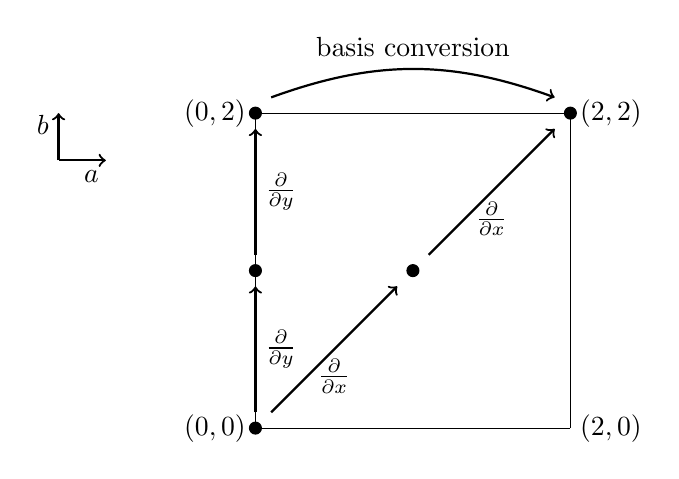
\begin{tikzpicture} 
% Box/square (4x4)
\draw[black,solid,ultra thin] (0,0)--(0,4);
\draw[black,solid,ultra thin] (0,0)--(4,0);
\draw[black,solid,ultra thin] (4,0)--(4,4);
\draw[black,solid,ultra thin] (0,4)--(4,4);
% Dots
\draw[black,fill=black] (0,0) circle (.5ex);
\draw[black,fill=black] (2,2) circle (.5ex);
\draw[black,fill=black] (4,4) circle (.5ex);
\draw[black,fill=black] (0,2) circle (.5ex);
\draw[black,fill=black] (0,4) circle (.5ex);
% Arrows
\draw[black,thick,->] (0.2,0.2)--(1.8,1.8);
\draw[black,thick,->] (2.2,2.2)--(3.8,3.8);
\draw[black,thick,->] (0,0.2)--(0,1.8);
\draw[black,thick,->] (0,2.2)--(0,3.8);
\draw [black,thick,->] (0.2,4.2) to [out=20,in=160] (3.8,4.2);
% Node (parameter) labels
\draw[] (0,0) node[anchor=east] {$(0,0)$};
\draw[] (0,4) node[anchor=east] {$(0,2)$};
\draw[] (4,0) node[anchor=west] {$(2,0)$};
\draw[] (4,4) node[anchor=west] {$(2,2)$};
% Arrow labels
\draw[] (1,1) node[anchor=north] {$\tfrac{\partial}{\partial x}$};
\draw[] (3,3) node[anchor=north] {$\tfrac{\partial}{\partial x}$};
\draw[] (0,1) node[anchor=west] {$\tfrac{\partial}{\partial y}$};
\draw[] (0,3) node[anchor=west] {$\tfrac{\partial}{\partial y}$};
% The key and headings
\draw[black,thick,->] (-2.5,3.4)--(-2.5,4);
\draw[black,thick,->] (-2.5,3.4)--(-1.9,3.4);
\draw[] (-2.3,3.2) node[anchor=west] {$a$};
\draw[] (-2.7,3.6) node[anchor=south] {$b$};
\draw[] (2,4.6) node[anchor=south] {basis conversion};
\end{tikzpicture} 
\caption{The Laplace operator acting on vectors of $P_{n,k}=P_{n,k}^{(0,0)}$ coefficients has a sparse matrix representation if the range is represented as vectors of $\smash{P^{(2,2)}_{n,k}}$ coefficients. Here, the arrows indicate that the corresponding operation has a sparse matrix representation when the domain is $\smash{P_{n,k}^{(a,b)}}$ coefficients, where $(a,b)$ is at the tail of the arrow, and the range is $\smash{P_{n,k}^{(\tilde{a},\tilde{b})}}$ coefficients, where $(\tilde{a},\tilde{b})$ is at the head of the arrow. %For example, $\smash{\frac{\partial}{\partial x}}$ has a sparse matrix representation when the domain is represented in $\smash{P_{n,k}^{(0,0,0)}}$ (resp.~$\smash{P_{n,k}^{(1,0,1)}}$) and the range in $\smash{P_{n,k}^{(1,0,1)}}$ (resp.~$\smash{P_{n,k}^{(2,0,2)}}$).
}
\label{fig:Laplace} 
\end{figure}

Firstly, we introduce further notation that
\begin{align}
\bigWab(x,y) := \Wab(x,y) \bigPab(x,y).
\end{align}

For general \(a,b\) and general functions \(f(x,y) = \bigPab(x,y)^\top \mathbf{f}\), there exist sparse operators \(D_x^{(a,b)}, \: D_y^{(a,b)}, \: W_x^{(a,b)}, \: W_y^{(a,b)}\) such that:
\begin{align}
\dx[f(x,y)] &= \bigP^{(a+1,b+1)}(x,y)^T \: D_x^{(a,b)} \: \mathbf{f}, \\
\dy[f(x,y)] &= \bigP^{(a,b+1)}(x,y)^T \: D_y^{(a,b)} \: \mathbf{f}, \\
\dx[\Wab(x,y) \: f(x,y)] &= \bigW^{(a-1,b-1)}(x,y)^T \: W_x^{(a,b)} \: \mathbf{f}, \\
\dy[\Wab(x,y) \: f(x,y)] &= \bigW^{(a,b-1)}(x,y)^T \: W_y^{(a,b)} \: \mathbf{f}.
\end{align}
The incrementing and decrementing of parameters as seen here is analogous to other well known orthogonal polynomials families' derivatives, for example the Jacobi polynomials, as seen in the DLMF \cite{DLMFDerivatives}.

Further, we note that there exist "parameter transformation" Banded-Block-Banded matrix operators that increment/decrement the parameters, transforming the OPs from one (weighted or non-weighted) parameter space to another. We denote these operators as $T_W^{(1,0)\to(0,0)}$, $T_W^{(1,1)\to(0,0)}$, $T^{(0,1)\to(1,1)}$, $T^{(0,2)\to(2,2)}$ and the general $T^{(a,b)\to(a+1,b+1)}$ where:
\begin{align}
\bigW^{(1,0)}(x,y) &= \Big(T_W^{(1,0)\to(0,0)} \Big)^T \: \bigP^{(0,0)}(x,y) \\
\bigW^{(1,1)}(x,y) &= \Big(T_W^{(1,1)\to(0,0)} \Big)^T \: \bigP^{(0,0)}(x,y) \\
\bigP^{(0,1)}(x,y) &= \Big(T^{(0,1)\to(1,1)} \Big)^T \: \bigP^{(1,1)}(x,y) \\
\bigP^{(0,2)}(x,y) &= \Big(T^{(0,2)\to(2,2)} \Big)^T \: \bigP^{(2,2)}(x,y) \\
\bigP^{(a,b)}(x,y) &= \Big(T^{(a,b)\to(a+1,b+1)} \Big)^T \: \bigP^{(a+1,b+1)}(x,y)
\end{align}

We can then obtain the matrix operator for \(\Delta\), that will take us from coefficients for expansion in the weighted space
\[
\bigWii(x,y) = \Wii(x,y) \: \bigPii(x,y)
\]
to coefficients in the non-weighted space
\[
\bigPii(x,y).
\]
Importantly, this operator will have Banded-Block-Banded structure, and hence will be sparse. Note that this construction will ensure the imposition of the Dirichlet zero boundary conditions on $\Omega$. The matrix operator \(\Delta\) acting on the coefficients vector is then given by
\begin{align}
    \Delta := D_x^{(0,0)} \: W_x^{(1,1)} + T^{(0,1)\to(1,1)} \: D_y^{(0,0)} \: T_W^{(1,0)\to(0,0)} \: W_y^{(1,1)}.
\end{align}

Further, we can also obtain the matrix operator for \(\Delta\) that will take us from coefficients for expansion in the space
\[
\bigPoo(x,y)
\]
to coefficients in the space
\[
\bigP^{(2,2)}(x,y).
\]
Importantly, again, this operator will have Banded-Block-Banded structure, and hence will be sparse. The matrix operator \(\Delta\) acting on the coefficients vector is then given by
\begin{align}
    D := D_x^{(1,1)} \: D_x^{(0,0)} + T^{(0,2)\to(2,2)} \: D_y^{(0,1)} \: D_y^{(0,0)}.
\end{align}

The sparsity of the these operators can be shown using a simply integration by parts argument, again showing that the sparsity for differential operators is not dependent on the domain.


\section{Computational aspects}

\subsection{Constructing $H_n^{(a,b)}(x)$}

????


\subsection{Quadrature rules}

In this section we construct a quadrature rule exact for polynomials in $\Omega$ that can be used to expand functions in $P_{n,k}^{(a,b)}(x,y)$. 

\begin{theorem}

Denote the  Gauss quadrature nodes and weight on \([0,1]\) with weight \(s^a \: (1-s^2)^{b+\half}\) as $(s_k,w_k^{(s)})$ , and
 on \([-1,1]\) with weight \((1-t^2)^b\) as $(t_k,w_k^{(t)})$. Define
\begin{align}
x_{i+(k-1)N} &:= s_k, \quad i,k = 1,\dots,N, \\
y_{l+(i-1)N} &:= (1-s_l^2)^\half \: t_l, \quad i,l = 1,\dots,N, \\
w_{l+(k-1)N} &:= w_k^{(s)} w_l^{(t)}, \quad k,l = 1,\dots,N.
\end{align}
If $f(x,y)$ is an at most degree $N$ polynomial in $x$ and at most degree $2N-1$ in $y$ then
$$
\iint_\Omega f(x,y) \: \Wab(x,y) \: \D A = \half \sum_{j=1}^{N^2} w_j \: \big[ f(x_j, y_j) + f(x_j, -y_j) \big],
$$

\end{theorem}
\begin{proof}

We will use the substitution that
\begin{align}
x &= s, \quad y = (1-s^2)^\half t.
\end{align}
First, note that
\begin{align}
W^{(a,b)}(x,y) &= x^a \: (1-x^2-y^2)^b, \quad \text{for } (x,y) \in \Omega, \\
		      &= s^a \: (1-s^2)^{b} \: (1-t^2)^b =: V^{(a,b)}(s,t), \quad \text{for } (s,t) \in [0,1] \times [-1,1].
\end{align}

\end{proof}




\subsection{Obtaining the coefficients for expansion of a function}

Fix \(a,b \in \R\). Then for any function \(f : \Omega \to \R\) of degree $N$ we can express \(f\) by
\begin{align*}
f(x,y) = \sum_{n=0}^N \bigP_n^{(a,b)}(x,y)^T \: \mathbf{f}_n
\end{align*}
where
\begin{align*}
\bigP_n(x,y) &:= \begin{bmatrix}
		P_{n,0}(x,y) \\
		\vdots \\
		P_{n,n}(x,y)
	\end{bmatrix} \in \R^{n+1} \quad \forall n = 0,1,2,\dots,N,
\end{align*}
and where
\begin{align*}
\mathbf{f}_n &:= \begin{bmatrix}
		f_{n,0} \\
		\vdots \\
		f_{n,n}
	\end{bmatrix} \in \R^{n+1} \quad \forall n = 0,1,2,\dots,N, \quad
f_{n,k} := \frac{\langle f, \: \Pnk^{(a,b)} \rangle_{W^{(a,b)}}}{|| \Pnk^{(a,b)} ||_{W^{(a,b)}}}
\end{align*}




We can develop a quadrature rule on the half disk \(\Omega\) in order to evaluate (40) and obtain the coefficient vectors \(\mathbf{f}_n\) as follows.




Let \(f(x,y)\) be polynomial that is even in \(y\) of degree $d_1$ in $x$ and degree $d_2$ in $y$ (i.e. $f(\cdot, y)$ with $y$ fixed is a degree $d_1$ polynomial, and $f(x, \cdot)$ with $x$ fixed is an even degree $d_2$ polynomial). Then there exists a polynomial \(\tilde{f}(x,y)\) in \(x,y\) such that \(g(s,t) := f(x, y) = f(s, (1-s^2)^\half t) = \tilde{f}(s, (1-s^2) t^2)\) (i.e. that $d_2$ is an even integer). Now, as \(\tilde{f}\) is a polynomial, so must \(g\) be a polynomial of degree $d_1+\frac{d_2}{2}$ in $s$ and degree $d_2$ in $t$. Thus a quadrature rule of the following will be exact for the polynomial $f(x,y)$ (even in \(y\) of degree $\le d_1$ in $x$ and degree $\le d_2$ in $y$):
\begin{align}
& \quad \int_0^1 \int_{-\rho(x)}^{\rho(x)} W^{(a,b)}(x,y) \: f(x,y) \: dy \: dx \\
&= \int_0^1 \int_{-1}^1 V^{(a,b)}(s,t) \: g(s,t) \: (1-s^2)^\half \: dt \: ds \\
&= \int_0^1 s^a \: (1-s^2)^{b+\half} \: \Big( \sum_k^{\half(d_2 + 1)} w_k^{(t)} \: g(s, t_k) \Big) \: ds \\
&= \sum_j^{\half(d_1 + \frac{d_2}{2} + 1)} \sum_k^{\half(d_2 + 1)} w_j^{(s)} w_k^{(t)} \: g(s_j, t_k) \\
&= \sum_j^{\half(d_1 + \frac{d_2}{2} + 1)} \sum_k^{\half(d_2 + 1)} w_j^{(s)} w_k^{(t)} \: f(x_j, y_{j,k}),
\end{align}
where \(x_j := s_j,\) \(y_{j,k} := \rho(s_j) \: t_k\) are the quadrature points.

We further note that for any polynomial \(f(x,y)\) that is odd in \(y\),
\begin{align}
\int_0^1 \int_{-\rho(x)}^{\rho(x)} W^{(a,b)}(x,y) \: f(x,y) \: dy \: dx = 0.
\end{align}


Then our quadrature rule for any polynomial \(f(x,y)\) on \(\Omega\) is:
\begin{align}
\int \int_\Omega W^{(a,b)}(x,y) \: f(x,y) \: dy \: dx \approx \half \: \sum_{j=1}^{N^2} w_j \: \big[ f(x_j, y_j) + f(x_j, -y_j) \big],
\end{align}
and is exact for any polynomial $f(x,y)$ where the degree in $x$ is $\le N$ and the degree in $y$ is $\le 2N-1$. Note that for a general polynomial where the overall degree is $N$, we still would hence need $N^2$ points and weights to make the rule exact. Thus,
\begin{align}
\ip< f, \: \Pnk^{(a,b)} >_{W^{(a,b)}} &= \half \: \sum_{j=1}^{N^2} w_j \: \big[ \big(f(x_j, y_j) \: \Pnk^{(a,b)}(x_j, y_j)\big) +\big(f(x_j, -y_j) \: \Pnk^{(a,b)}(x_j, -y_j)\big) \big], \\
|| \Pnk^{(a,b)} ||_{W^{(a,b)}}^2 &= \half \: \sum_{j=1}^{N^2} w_j \: \big[ \Pnk^{(a,b)}(x_j, y_j)^2 + \Pnk^{(a,b)}(x_j, -y_j)^2 \big],
\end{align}
for suitably large $N$.


%
\section{Examples on the half disk with zero BCs}


\subsection{Poisson}

\begin{figure}
	\centering
	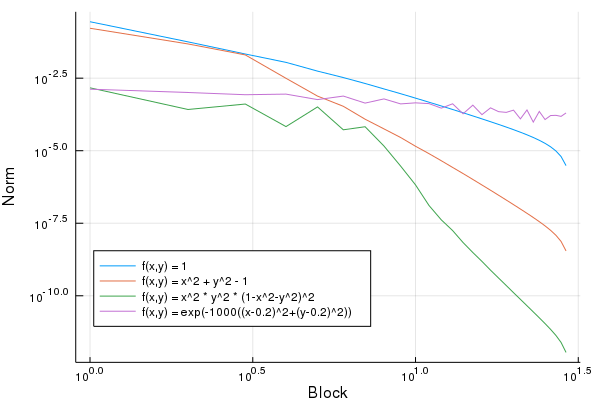
\includegraphics[scale=0.4]{solutionblocknorms}
	\caption{The norms of each block of the computed solution of the Poisson equation with the given right hand side functions.}
	\centering
	\label{fig:solutionblocknorms}
\end{figure}

Find \(u(x,y)\) given a function \(f(x,y)\) such that:
\begin{align}
	\begin{cases}
    		\Delta u(x,y) = f(x,y) \quad \text{in } \Omega \\
		u(x,y) = 0 \quad \text{on } \partial \Omega
	\end{cases}.
\end{align}
noting the imposition of zero Dirichlet boundary conditions on $u$.

We can tackle the problem as follows. Fix \(a, b = 1,1\). Denote the coefficient vector for expansion of $u$ in the $\bigWii$ OP basis up to degree $N$ by $\mathbf{u}$, and the coefficient vector for expansion of $f$ in the $\bigPii$ OP basis up to degree $N$ by $\mathbf{f}$. Since $f$ is known, we can obtain $\mathbf{f}$ using the quadrature rule above. In matrix-vector notation, our system hence becomes:
\begin{align}
    \Delta^{(1,1)} \mathbf{u} = \mathbf{f}
\end{align}
which can be solved to find $\mathbf{u}$.

%\begin{figure}
%	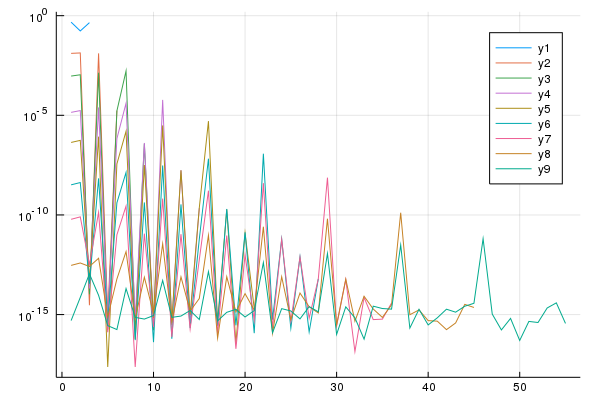
\includegraphics[scale=0.4]{example4coeffs}
%\centering
%\caption{Plot of the difference between the previous solution's coefficients and the current solution's coefficients under increasing degree of approximation (number of coefficients used) for $N = 2,\dots,10$, using RHS of $f(x,y) = 2(1-x^2-y^2)\cos(x) - 8x\sin(x) - x(1-x^2-y^2)\sin(x) - 4x^2 \cos(x) - 12xy$ for the Poisson equation. The solution is converging as seen by the decreasing (absolute value) difference of coefficient values.}
%\centering
%\label{fig:poisson}
%\end{figure}

\begin{figure}
	\centering
	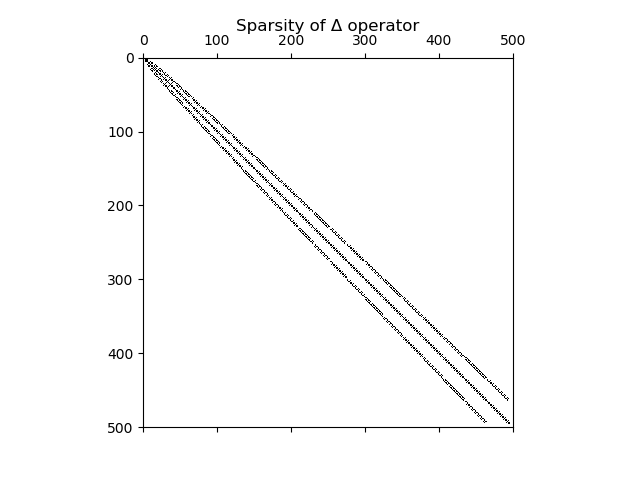
\includegraphics[scale=0.4]{sparsityoflaplacian}
        \label{fig:sparsity}
    	\caption{A "spy" plot of the $\Delta$ operator for $\bigWii(x,y) \to \bigPii(x,y)$ showing its sparsity.}
	\centering
\end{figure}

\subsection{Inhomogenous Helmholtz}

Find \(u(x,y)\) given a function \(f(x,y)\) such that:
\begin{align}
	\begin{cases}
    		\Delta u(x,y) + k^2 u(x,y) = f(x,y) \quad \text{in } \Omega \\
		u(x,y) = 0 \quad \text{on } \partial \Omega
	\end{cases}.
\end{align}
noting the imposition of zero Dirichlet boundary conditions on $u$.

We can tackle the problem as follows. Fix \(a, b = 1,1\). Denote the coefficient vector for expansion of $u$ in the $\bigWii$ OP basis up to degree $N$ by $\mathbf{u}$, and the coefficient vector for expansion of $f$ in the $\bigPii$ OP basis up to degree $N$ by $\mathbf{f}$. Since $f$ is known, we can obtain $\mathbf{f}$ using the quadrature rule above. In matrix-vector notation, our system hence becomes:
\begin{align}
    (\Delta^{(1,1)} + k^2 T^{(0,0)\to(1,1)} T_W^{(1,1)\to(0,0)}) \mathbf{u} = \mathbf{f}
\end{align}
which can be solved to find $\mathbf{u}$.

We can extend this to constant non-zero boundary conditions by simply noting that the problem 
\begin{align}
	\begin{cases}
    		\Delta u(x,y) + k^2 u(x,y) = f(x,y) \quad \text{in } \Omega \\
		u(x,y) = c \in \R \quad \text{on } \partial \Omega
	\end{cases}
\end{align}
is equivalent to letting $u = v + c$ and solving
\begin{align}
	\begin{cases}
    		\Delta v(x,y) + k^2 v(x,y) = f(x,y) - k^2 c =: g(x,y)  \quad \text{in } \Omega \\
		v(x,y) = 0 \quad \text{on } \partial \Omega
	\end{cases}.
\end{align}

\begin{figure}
	\centering
	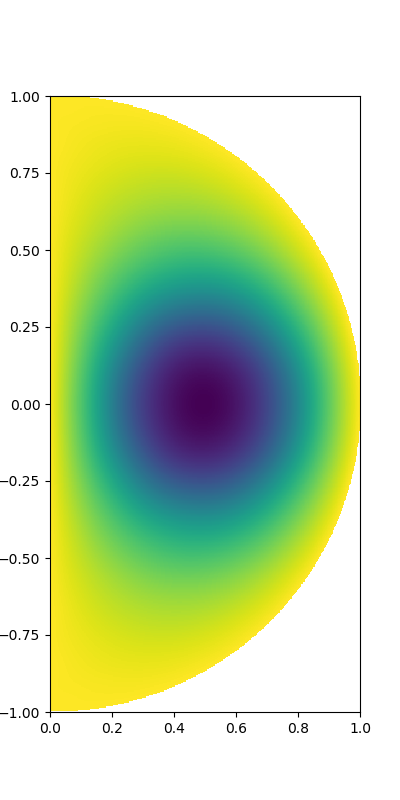
\includegraphics[scale=0.3]{solution}
        	\label{fig:solution}
    	\caption{The computed solution to $\Delta u = f$ with zero boundary conditions with $f(x,y) = 1 + \text{erf}(5(1 - 10((x - 0.5)^2 + y^2)))$.}
	\centering
\end{figure}

\subsection{Heat Equation}
Consider
\begin{align}
	\begin{cases}
		\frac{\partial u}{\partial t}(t,x,y) = \Delta u(t,x,y) \quad \text{in } \Omega \\
		u(t, x, y) = 0 \quad \text{on } \partial \Omega \\
		u(0, x, y) = u_0(x,y) := \Wii(x,y) \: f(x,y)
	\end{cases}
\end{align}
noting the imposition of zero Dirichlet boundary conditions.

Using a backward Euler time-stepping method, we can formulate this for \(t = 0,1,2,\dots\) and step length $h$:
\begin{align}
u_{t+1}(x,y) - u_t (x,y) = h \: \Delta u_{t+1}(x,y) \quad \text{for } (x,y) \in \Omega.
\end{align}

We can tackle the problem as follows. Fix \(a, b = 1,1\). Denote the coefficient vector for expansion of $u_0$ in the $\bigWii$ OP basis up to degree $N$ by $\mathbf{u}_0$, and similarly for each $t = 1,2,3,\dots,t_{max}$ we denote $\mathbf{u}_t$ as the coefficient vector of the expansion of $u_t$ in the $\bigWii$ OP basis up to degree $N$. Further, denote the coefficient vector for expansion of $u_0$ in the $\bigPii$ OP basis up to degree $N$ by $\mathbf{\tilde{u}}_0$, and similarly for each $t = 1,2,3,\dots,t_{max}$ denote $\mathbf{\tilde{u}}_t$ as the coefficient vector of the expansion of $u_t$ in the $\bigPii$ OP basis up to degree $N$.

Then, using the operator $\Delta$, we can solve this system for the given initial condition $\mathbf{u_0}$ by iterating for $t = 0,1,2,\dots,t_{max}$:
\begin{align}
	&T^{(0,0)\to(1,1)} \: T_W^{(1,1)\to(0,0)} \: (\mathbf{u}_{t+1} - \mathbf{u}_t) = h \: \Delta^{(1,1)} \mathbf{u}_{t+1} \nonumber \\
	\iff& (T^{(0,0)\to(1,1)} \:T_W^{(1,1)\to(0,0)} - h \: \Delta^{(1,1)}) \: \mathbf{u}_{t+1} = T^{(0,0)\to(1,1)} \: T_W^{(1,1)\to(0,0)} \: \mathbf{u}_t \nonumber \\
	\iff& \mathbf{u}_{t+1} = (T^{(0,0)\to(1,1)} \: T_W^{(1,1)\to(0,0)} - h \: \Delta^{(1,1)})^{-1} T^{(0,0)\to(1,1)} \: T_W^{(1,1)\to(0,0)} \: \mathbf{u}_t \nonumber \\
	\iff& \mathbf{\tilde{u}}_{t+1} = T^{(0,0)\to(1,1)} \: T_W^{(1,1)\to(0,0)} \: (T^{(0,0)\to(1,1)} \: T_W^{(1,1)\to(0,0)} - h \: \Delta^{(1,1)})^{-1} \: \mathbf{\tilde{u}}_t.
\end{align}

%\begin{figure}
%	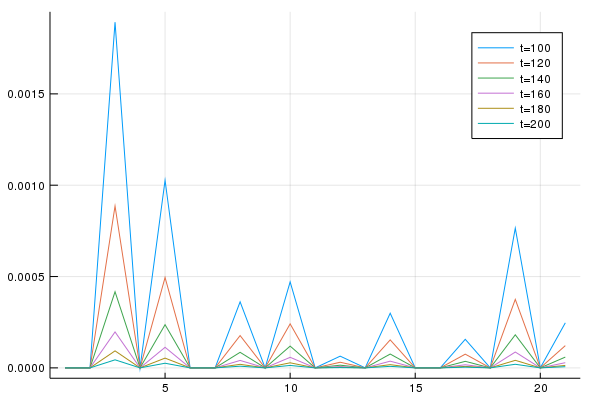
\includegraphics[scale=0.4]{example2timesteppingcovnvergence}
%\centering
%\caption{Plot of the current iteration's coefficients for the heat equation example, using degree of approximation $N = 5$ with initial condition of $u_0(x,y) = \Wii(x,y)$ and step size $h=0.01$, plotted for iterations $t=100, 120, \dots, 200$. The solution tends to zero, as seen by the decreasing (absolute value) coefficient values.}
%\centering
%\label{fig:heateqn}
%\end{figure}



%
\section{Future work - orthogonal polynomials on the hemisphere and spherical triangles}

We will use a similar idea of projecting up from 1D OPs to the interval, to 2D OPs on the disk, to 3D OPs on the sphere. Initially, we will add to the ApproxFun library by adding capability to work with OPs on the half disk (2D) with weights governed by parameters that will be incremented/decremented after an application of an operator (e.g. partial derivative). With this, we can obtain a family of OPs on the hemisphere, with sparse relations.

Beyond this, solving PDEs on isosceles triangles should follow using the same procedure. However, we are expecting that to solve PDEs on spherical triangles (as is our ultimate goal) will require further ideas beyond the procedures given in this document.

%
\appendix
%
\section{P-finite element methods using sparse operators}

We follow the method of \cite{beuchler2006new}. Consider the 2D Dirichlet problem on a domain $\Omega$:
\begin{align}
	\begin{cases}
         - \Delta u(x,y) = f(x,y) \quad \text{in } \Omega \\
         u = 0 \quad \text{on } \partial \Omega
         \end{cases}
\end{align}
This has the weak formulation for any test function $v \in V := H_0^1(\Omega) = \{v \in H^1(\Omega) \quad | \quad v|_{\partial \Omega} = 0 \}$,
\begin{align}
	L(v) := \int_\Omega f \: v \: d\mathbf{x} = \int_\Omega \nabla u \cdot \nabla v \: d\mathbf{x} =: a(u,v).
\end{align}

In general, we would let $\FEset$ be the set of elements $\element$ that make up our finite element discretisation of the domain, where each $\element$ is a rhombus or disk slice for example. 

\subsection{Single element p-FEM}
In this section, we limit our discretisation to a single element, that is we let $\element = \Omega$ for a half disk/disk slice/rhombus domain. We can choose our finite dimensional space $V_h = \{v_h \in V \quad | \quad deg(v_h|_\element) \le p\}$ for some $p \in \N$.

We seek $u_h \in V_h$ s.t.
\begin{align}
	L(v_h) = a(u_h,v_h) \quad \forall \: v_h \in V_h.
\end{align}

Define $\Lambda^{(a,b)} := \langle \bigP^{(a,b)}, \: {\bigP^{(a,b)}}^T \rangle_{W^{(a,b)}}$ where $W^{(a,b)}$ is the weight with which the OPs in $\bigP^{(a,b)}$ are orthogonal with respect to. Note that due to orthogonality this is a diagonal matrix. We can choose a basis for $V_h$ by using the weighted orthogonal polynomials on $\element$ with parameters $a = b = 1$:
\begin{align}
\bigWii(x,y) &:= \begin{bmatrix}
		\bigWii_0(x,y) \\
		\bigWii_1(x,y) \\
		\bigWii_2(x,y) \\
		\vdots \\
		\bigWii_p(x,y)
	\end{bmatrix}, \\
\bigWii_n(x,y) &:= \begin{bmatrix}
		\Wii(x,y) \: \Pii_{n,0}(x,y) \\
		\vdots \\
		\Wii(a,y) \: \Pii_{n,n}(x,y)
	\end{bmatrix} \in \R^{n+1} \quad \forall n = 0,1,2,\dots,p,
\end{align}
and rewrite (73) in matrix form:
\begin{align}
	a(u_h,v_h) &= \int_\element \nabla u_h \cdot \nabla v_h \: d\mathbf{x} \\
	&= \int_\element \begin{bmatrix}
					\partial_x v_h \\
					\partial_y v_h
				\end{bmatrix}^T 
				\begin{bmatrix}
					\partial_x u_h \\
					\partial_y u_h
				\end{bmatrix}
				\\
	&= \int_\element \begin{bmatrix}
					\bigPoo^T \Wii_x \mathbf{v} \\
					\bigPoo^T T^{(1,0)\to(0,0)} \Wii_y \mathbf{v}
				\end{bmatrix}^T 
				\begin{bmatrix}
					\bigPoo^T \Wii_x \mathbf{u} \\
					\bigPoo^T T^{(1,0)\to(0,0)} \Wii_y \mathbf{u}
				\end{bmatrix}
				\\
	&= \int_\element \Big( \mathbf{v}^T {\Wii_x}^T \bigPoo \bigPoo^T \Wii_x \mathbf{u} \nonumber \\
					& \quad \quad \quad + \mathbf{v}^T ({T^{(1,0)\to(0,0)} \Wii_y})^T \bigPoo \bigPoo^T T^{(1,0)\to(0,0)} \Wii_y \mathbf{u}  \Big) \: d\mathbf{x} \\
	&= \mathbf{v}^T \: \Big( {\Wii_x}^T \Lambda^{(0,0)} \Wii_x + ({T^{(1,0)\to(0,0)} \Wii_y})^T \Lambda^{(0,0)} T^{(1,0)\to(0,0)} \Wii_y \Big) \: \mathbf{u}
\end{align}
where $\mathbf{u}, \mathbf{v}$ are the coefficient vectors of the expansions of $u_h, v_h \in V_h$ respectively in the $V_h$ basis ($\bigWii$ OPs), and
\begin{align}
	L(v_h) &= \int_\element \: v_h \: f \: d\mathbf{x} \\
	&= \int_\element \: \mathbf{v}^T \: \bigWii \: \bigPii^T \: \mathbf{f} \: d\mathbf{x} \\
	&= \mathbf{v}^T \: \langle \bigPii, {\bigPii}^T \rangle_{\Wii} \: d\mathbf{x} \\
	&= \mathbf{v}^T \Lambda^{(1,1)} \: \mathbf{f},
\end{align}
where $\mathbf{f}$ is the coefficient vector for the expansion of the function $f(x,y)$ in the $\bigPii$ OP basis.

Since (73) is equivalent to stating that
\begin{align}
	L(\Wii \Pii_{n,k}) = a(u_h,\Wii \Pii_{n,k}) \quad \forall \: n = 0,\dots,p, \: k = 0,\dots,n,
\end{align}
(i.e. holds for all basis functions of $V_h$) by choosing $v_h$ as each basis function, we can equivalently write the linear system for our finite element problem as:
\begin{align}
A\mathbf{u} = \tilde{\mathbf{f}}.
\end{align}
where the (element) stiffness matrix $A$ is defined by 
\begin{align}
A = {\Wii_x}^T \Lambda^{(0,0)} \Wii_x + ({T^{(1,0)\to(0,0)} \Wii_y})^T \Lambda^{(0,0)} T^{(1,0)\to(0,0)} \Wii_y, 
\end{align}
and the load vector $\tilde{\mathbf{f}}$ is given by 
\begin{align}
\tilde{\mathbf{f}} = \Lambda^{(1,1)} \: \mathbf{f}.
\end{align}

Note the since we have sparse operator matrices for partial derivatives and basis-transform, we obtain a symmetric sparse (element) stiffness matrix, as well as a sparse operator matrix for calculating the load vector (rhs).

\subsection{Two-element p-FEM on the disk (without BCs)}
We now consider the case of using two elements to discretise a unit disk domain $\Omega$, that is the each element $\element$ is a half-disk, with common edge defined by the line $x=0$ for $y \in [-1,1]$. We take inspiration from \cite{karniadakis2013spectral, beuchler2006new}. To ensure continuity across the edge interface, we need to expand our basis functions to be used. We require basis functions that correspond to each edge (in this case there is only one edge), that is basis functions with support as the two elements connected by said edge (for more than two elements - and hence more than one edge - we would also stipulate that each edge's corresponding basis functions would vanish on any other edge). We then also require the remaining (interior) basis functions be such that they have support of one element only, and vanish on (each) edge. Using this, our basis functions for $\le N$-degree polynomials can then be written as
\begin{align}
	\bigQab_n(x,y) := \begin{bmatrix}
		P^{(a,b)}_{n,n}(x,y) \\
		x \: \bigPab_{n-1}(x,y)
	\end{bmatrix} \in \R^{n+1}, 
	\quad \quad 
	\bigQab := \begin{bmatrix}
		\bigQab_0 \\
		\bigQab_1 \\
		\vdots \\
		\bigQab_N
	\end{bmatrix}.
\end{align}
We note that for each $n = 0,\dots,N$, $P^{(a,b)}_{n,n}(x,y) = \rho(x)^n \: P^{(a,b)}_{n}(\frac{y}{\rho(x)})$ and so at $x=0$ these become just the Jacobi polynomials in $y$, thus span the edge interface. The polynomials that make up the $\bigQab$ basis can also be shown to have similar sparse relations and yield similar sparse operator matrices. We can then proceed to use a similar approach to section A.1 on a reference element.


\section{Disk slices}

The work in this paper on the half disk can be easily transferred to the domain of a disk slice by which we mean
\begin{align}
	\Omega := \{(x,y) \in \R^2 \quad | \quad \alpha < x < \beta, \: \gamma \rho(x) < y < \delta \rho(x)\}
\end{align}
with 
\begin{align}
\begin{cases}
-1 \le \alpha < &\beta \le 1 \\
(\gamma, \delta) &:= (-1,1) \\
\rho(x) &:= (1-x^2)^{\half} \\
w^{(a,b,c)}_1(x) &:= (\beta - x)^a \: (x - \alpha)^{b} \: \rho(x)^{2c} = (\beta - x)^a \: (x - \alpha)^{b} \: (1-x^2)^{c} \\
w^{(b)}_2(x) &:= (1-x^2)^b = (1-x)^b \: (1+x)^b.
\end{cases}
\end{align}
The weight $w^{(b)}_2(x)$ is a still an ultraspherical weight, and the corresponding OPs are the Jacobi polynomials $\{P_n^{(b, b)}\}$. $w^{(a,b,c)}_1(x)$ is the (non-classical) weight for the OPs denoted $\{H_n^{(a, b,c)}\}\). Thus we arrive at the two parameter family of 2D orthogonal polynomials $\{\Pnk\}$ on $\Omega$ given by, for \(0 \le k \le n, \: n = 0,1,2,\dots,\)
\begin{align}
	\Pnk^{(a,b,c)}(x,y) := H_{n-k}^{(c, a, b+k+\half)}(x) \: \rho(x)^k \: P_k^{(b,b)}(\frac{y}{\rho(x)}), \quad (x,y) \in \Omega, 
\end{align}
orthogonal with respect to the weight
\begin{align}
	W^{(a,b,c)}(x,y) &:= w^{(c,a,b)}_1(x) w^{(b)}_2(\frac{y}{\rho(x)}) \nonumber \\
	&= (\beta - x)^c \: (x - \alpha)^{a} \: (\rho(x)^2 -y^2)^b \nonumber \\
	&= (\beta - x)^c \: (x - \alpha)^{a} \: (1 - x^2 -y^2)^b , \quad (x,y) \in \Omega.
\end{align}

Note that by setting $c = 0$, $\alpha = 0$ and $\beta = 1$ we obtain the 2D orthogonal polynomials on the half disk.


\section{Hemisphere}

We can use the similar idea of projecting up from the 2D orthogonal polynomials on the half disk to 3D OPs on the hemisphere. Define $\rho(x) := (1-x^2)^\half$ for $x \in [0,1]$ and let the half disk be denoted by $\omega$, that is let
\begin{align}
	\omega := \{(x,y) \in \R^2 \quad | \quad 1 < x < 0, \: \rho(x) < y < \rho(x)\}.
\end{align}
Further, define the hemisphere by
\begin{align}
	\Omega := \{(x,y,z) \in \R^3 \quad | \quad (x,y) \in \omega, \: x^2 + y^2 + z^2 = 1\}.
\end{align}
We can define the 3D OP family on the hemisphere as the set of polynomials $\bigQab(x,y,z)$ where
\begin{align}
	\bigQab_n(x,y,z) := \begin{bmatrix}
		\bigPab_n(x,y) \\
		z \: \bigP^{(a,b+1)}_{n-1}(x,y)
	\end{bmatrix} \in \R^{2n+1}, 
	\quad \quad 
	\bigQab := \begin{bmatrix}
		\bigQab_0 \\
		\bigQab_1 \\
		\vdots \\
		\bigQab_N
	\end{bmatrix}.
\end{align}
The relations for multiplication by $x, y$ are then trivial. For multiplication by $z$, note that $z^2 = W^{(0,1)}(x,y)$ for $(x,y,z) \in \Omega$ and consider that (as the 2D OPs for any parameters form a 2D basis of $\omega$):
\begin{align}
	z \: \Pnkab(x,y) &= \sum_{m,j} c_{n,k,m,j}^{(a,b)\to(a,b+1)} \: z \: P^{(a,b+1)}_{m,j}(x,y), \\
	z^2 \: \Pnkab(x,y) &= \sum_{m,j} d_{n,k,m,j}^{(a,b)\to(a,b-1)} \: z \: P^{(a,b-1)}_{m,j}(x,y).
\end{align}
A simple calculation shows that the expansions are sparse, that is that most coefficients $c_{n,k,m,j}^{(a,b)\to(a,b+1)}$ and $d_{n,k,m,j}^{(a,b)\to(a,b-1)}$ are $0$, and are also given by
\begin{align}
	c_{n,k,m,j}^{(a,b)\to(a,b+1)} &= \frac{\ip< \Pnkab, \: P^{(a,b+1)}_{m,j} >_{W^{(a,b+1)}}}{\norm{P^{(a,b+1)}_{m,j}}^2_{W^{(a,b+1)}}} \\
	d_{n,k,m,j}^{(a,b)\to(a,b-1)} &= \frac{\ip< W^{(0,1)} \Pnkab, \: P^{(a,b-1)}_{m,j} >_{W^{(a,b-1)}}}{\norm{P^{(a,b-1)}_{m,j}}^2_{W^{(a,b-1)}}} \nonumber \\
	&= \frac{\ip< \Pnkab, \: P^{(a,b-1)}_{m,j} >_{W^{(a,b)}}}{\norm{P^{(a,b-1)}_{m,j}}^2_{W^{(a,b-1)}}} \nonumber \\
	&= \frac{\norm{\Pnkab}_\Wab^2}{\norm{P^{(a,b-1)}_{m,j}}^2_{W^{(a,b-1)}}} \: c_{m,j,n,k}^{(a,b-1)\to(a,b)}.
\end{align}
The coefficients $c_{n,k,m,j}^{(a,b)\to(a,b+1)}$ and $d_{n,k,m,j}^{(a,b)\to(a,b-1)}$ are just the entries to the parameter tranformation operator matrices
\begin{align}
	\bigP^{(a,b)}(x,y) &= \Big(T^{(a,b)\to(a,b+1)} \Big)^T \: \bigP^{(a,b+1)}(x,y) \\
	W^{(0,1)}(x,y) \bigP^{(a,b)}(x,y) &= \Big(T^{(a,b)\to(a,b-1)} \Big)^T \: \bigP^{(a,b-1)}(x,y)
\end{align}
respectively.




\bibliography{halfdisk-bib}


\end{document}











  